\chapter{Implementasi dan Pengujian Sistem HILS}\label{chapter-4}

\section{Implementasi Sistem HILS}

Berdasarkan analisis dan rancangan solusi pada Bab \ref{chapter-3}, dapat
dimulai implementasi sistem HILS baru. Implementasi sistem HILS dimulai dengan
eksplorasi ROS2 dan ZeroMQ. Kemudian dilanjutkan dengan pembuatan program
\textit{proof of concept} (POC) menggunakan salah satu mekanisme komunikasi.
POC dibuat untuk menunjukan bahwa mekanisme komunikasi yang digunakan dapat
melakukan transfer data kamera sehingga CARLA berjalan dengan setidaknya 2 FPS.
Setelah POC diterima oleh ketua tim simulasi, dilanjutkan penulisan pustaka
\textit{consumer} dan terakihir implementasi pustaka \textit{producer}.

Dari proses eksplorasi dan implementasi POC, didapatkan metode komunikasi yang
cocok adalah ZeroMQ. ROS 2 sendiri gagal pada tahap POC dikarenakan sistem
operasi tidak kompatibel dengan ROS 2. Oleh karena itu, implementasi pustaka
akan menggunakan ZeroMQ. Sedangkan, ROS 2 tidak akan digunakan lagi pada tugas
akhir ini.

Pustaka yang pertama ditulis adalah pustaka \textit{consumer} (sisi
komputer AGX/RKB) karena program utama komputer SILS (pengguna
\textit{producer}) belum selesai pada saat proses penulisan pustaka. Akibatnya,
pengujian pustaka \textit{consumer} lebih mudah dilakukan pada saat itu.

Pustaka \textit{producer} dan \textit{consumer} akan memanfaatkan pemrograman
berorientasi objek untuk menstruktur kodenya. Pustaka yang dibuat juga dibuat
seabstrak mungkin dan tidak \textit{coupled} pada trem saja. Sehingga pustaka
yang ditulis dapat digunakan untuk simulasi \textit{hardware-in-the-loop} jenis
kendaraan otonom lainnya.

Diagram kelas dari pustaka \textit{consumer} dapat dilihat pada gambar
\ref{chapter-4-consumer-class-diagram}. Kelas yang melakukan komunikasi adalah
kelas abstrak \texttt{Endpoint}. Kelas tersebut dibuat abstrak dan diinstansiasi
menggunakan pola pemrograman \textit{factory}. \texttt{Endpoint} dibuat abstrak
agar apabila ingin ditambahkan metode komunikasi lain, hal tersebut dapat
dilakukan dengan mudah. Contoh kasus penggunaan penambahan metode komunikasi
lain adalah pengujian atau \textit{benchmarking} metode komunikasi. Selain itu,
terdapat kelas yang akan menyediakan layanan untuk program GRS, yaitu
\texttt{CarlaService}. Kelas ini mengabstraksi komunikasi dan deserialisasi
ataupun serialisasi data dari \texttt{Endpoint}.

\begin{figure}[!htbp]
	\centering
	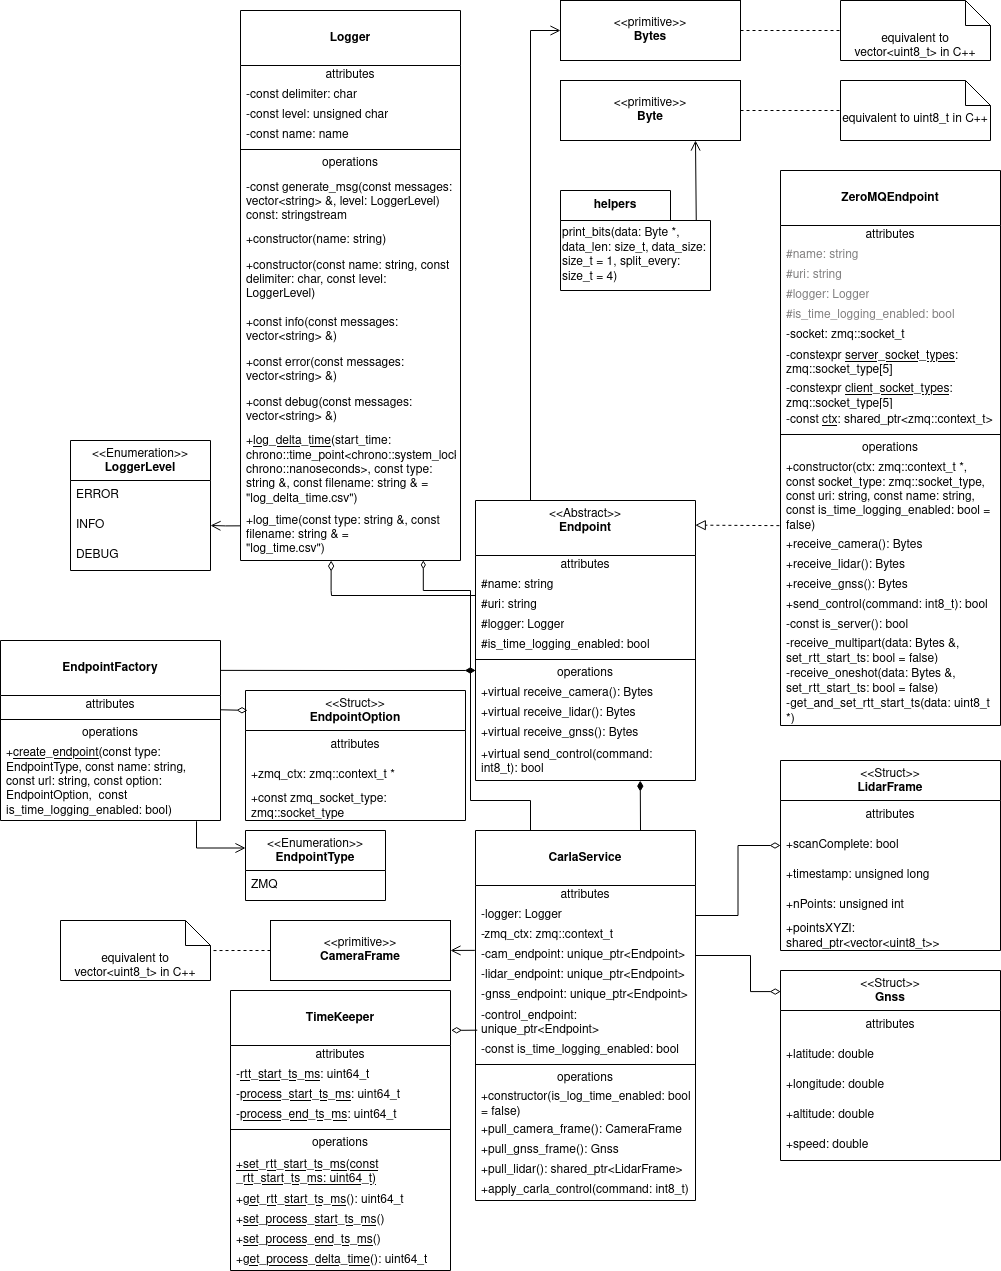
\includegraphics[width=1.0\textwidth]{resources/chapter-4/consumer-class_diagram.png}
	\caption{Diagram Kelas Pustaka \textit{Consumer}}
	\label{chapter-4-consumer-class-diagram}
\end{figure}

Setelah pustaka \textit{consumer} berhasil, implementasi dilanjutkan dengan
pembuatan pustaka \textit{producer}. Diagram kelas pustaka \textit{producer}
dapat dilihat pada gambar \ref{chapter-4-producer-class-diagram}. Pembuatan
pustaka \textit{producer} juga mengikuti filosofi penulisan pustaka
\textit{consumer}. Pustaka dibuat seabstrak mungkin sehingga tidak
\textit{coupled} dengan trem. Kelas \texttt{Endpoint} juga dibuat abstrak agar
dapat ditambahkan metode komunikasi yang lain. Perbedaan implementasi adalah
pada kelas yang berinteraksi dengan program utama. Pada pustaka
\textit{producer}, ada empat kelas yang berinteraksi dengan program utama, yaitu
\texttt{CameraHandler}, \texttt{LidarHandler}, \texttt{GnssHandler}, dan
\texttt{ControlHandler}. Keempat kelas memiliki peran masing-masing dan
terspesialisasi untuk menangani data dari sensor virtual CARLA tertentu.

\begin{figure}[!htbp]
	\centering
	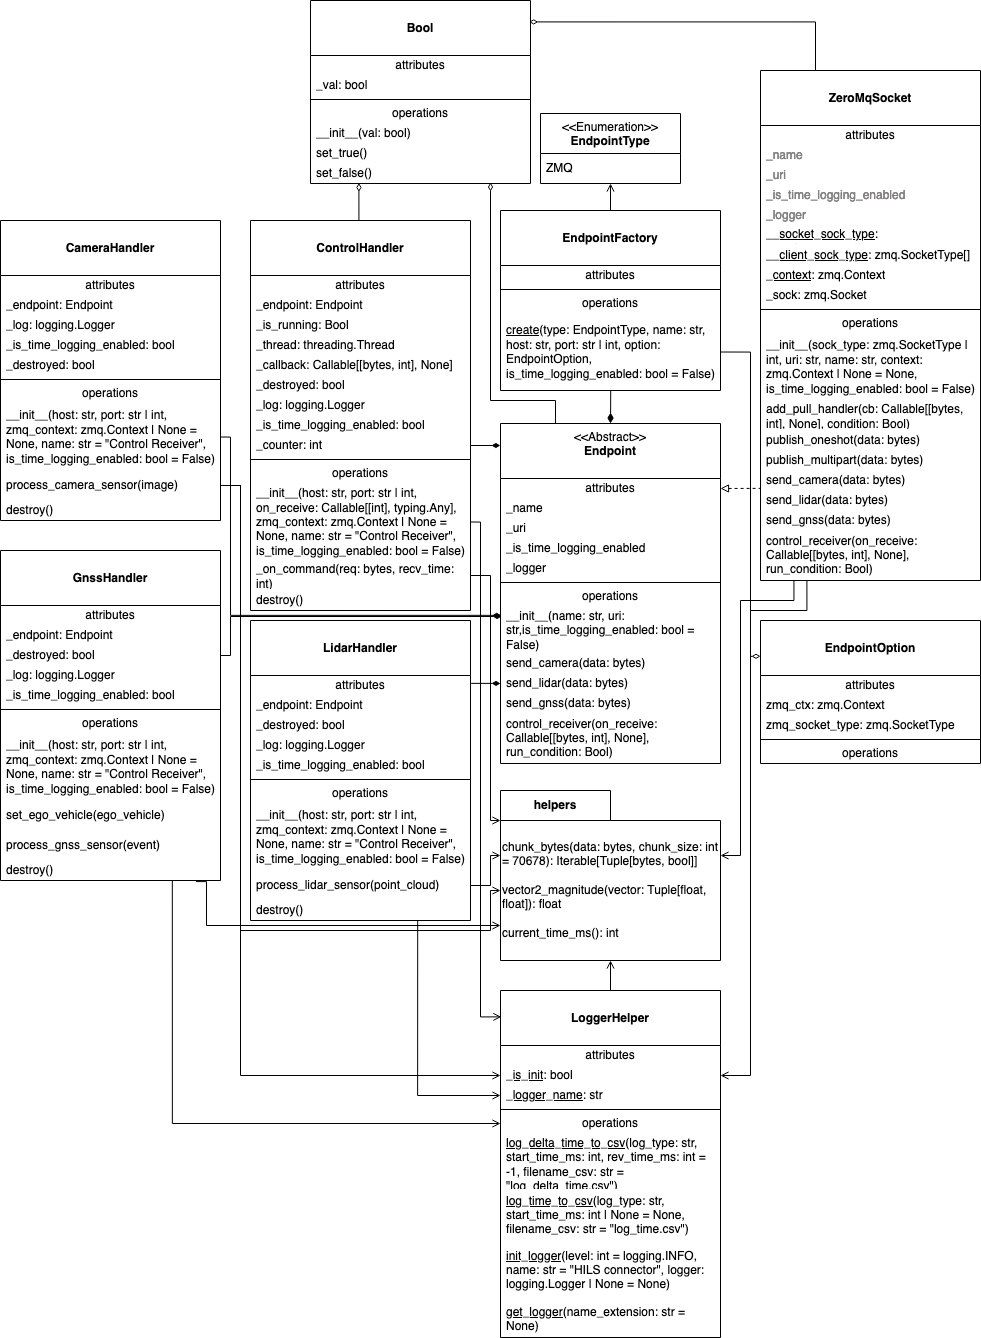
\includegraphics[width=1.0\textwidth]{resources/chapter-4/producer-class_diagram.png}
	\caption{Diagram Kelas Pustaka \textit{Producer}}
	\label{chapter-4-producer-class-diagram}
\end{figure}

Setelah kedua pustaka diimplementasi, dilakukan pengujian pustaka dengan program
kecil. Lalu, kedua pustaka diintegrasi dengan kedua program utama. Setelah itu,
dapat dianggap sistem implementasi HILS yang baru sudah diimplementasi dan
pengujian HILS dapat dilakukan. Akan tetapi untuk kebutuhan tugas akhir, sebelum
pengujian HILS dilakukan, akan dilaksanakan pengujian. Metode pengujian dan
aspek sistem yang diuji akan dibahas pada Subbab
\ref{chapter-4-testing-methodology}.

\section{Metode Pengujian Implementasi dan
  Kinerja}\label{chapter-4-testing-methodology}

Pengujian akan menguji dua aspek, yaitu
\begin{enumerate}
	\item pengujian implementasi: meninjau kemampuan sistem HILS dalam mengirim,
	      menerima, dan menggunakan data dari sensor; dan
	\item pengujian kinerja: meninjau latensi yang dibutuhkan untuk mengirim
	      data.
\end{enumerate}
Bagian ini, Subbab \ref{chapter-4-testing-methodology}, akan membahas metode dan
rencana pengujian kedua aspek tersebut. Pengujian dilakukan dengan menjalankan
beberapa skenario simulasi lalu dibandingkan dengan kriteria kedua aspek. Sebuah
aspek dinyatakan berhasil/lolos apabila semua kriterianya berhasil dicapai.

\subsection{Pengujian Implementasi Sistem HILS}

Pengujian implementasi dilakukan dengan menjalankan program utama di komputer
SILS dan komputer AGX/RKB. Kemudian, akan dilakukan observasi untuk memeriksa
sistem HILS sudah memenuhi kriteria-kriteria berikut atau belum.

\begin{enumerate}
	\item kecepatan trem di program GRS sesuai dengan bacaan sensor GNSS,
	\item tampilan kamera di program GRS sesuai dengan yang ada di program
	      ScenarioRunner,
	\item tampilan lidar di program GRS menggambarkan objek-objek yang ada di
	      sekitar trem,
	\item trem dapat maju atau berhenti tanpa masukan dari papan ketik, dan
	\item trem maju ketika mendapatkan kendali maju dan berhenti ketika
	      mendapatkan kendali berhenti.
\end{enumerate}

Kriteria ini selaras dengan tujuan tugas akhir yang kedua, yaitu
mengimplementasikan sistem simulasi yang dapat mengirimkan, menerima, dan
memanfaatkan data dari berbagai jenis sensor.

\subsection{Pengujian Kinerja Sistem HILS}

Dari segi kinerja, hal yang ingin dipastikan adalah CARLA dapat berjalan dengan
stabil dan kecepatan minimum 2 FPS (\textit{frames per second}). Hal tersebut
diobservasi dengan menjalankan kedua program utama. Selain dari kecepatan
simulator, aspek kinerja juga akan dinilai dari perbandingan dengan implementasi
HILS sebelumnya. Latensi pengiriman data harus lebih rendah dibandingkan latensi
implementasi HILS sebelumnya.

Untuk kriteria kedua, pengujian latensi implementasi HILS sebelumnya akan
dilakukan secara teoretis. Hal ini karena implementasi HILS sebelumnya sudah
sulit untuk dijalankan. Selain itu, jenis data yang dikirim pada implementasi
HILS sebelumnya juga berbeda. Pengujian secara teoretis ini dilakukan dengan
menulis ulang sebagian dari mekanisme komunikasi implementasi HILS sebelumnya.
Bagian yang akan ditulis ulang adalah operasi pembacaan data dari \textit{file},
penulisan dan pembacaan ke basis data, serta penulisan data sensor yang dibaca
dari basis data ke \textit{file}. Dengan demikian, ada 4 operasi I/O dari
implementasi HILS sebelumnya yang ditulis ulang untuk pengujian latensi secara
teoretis.

Apabila sistem HILS berhasil memenuhi kedua kriteria tersebut, sistem dapat
dianggap sudah berhasil memenuhi kedua tujuan tugas akhir. Hal tersebut karena
kinerja sistem akan dipengaruhi mekanisme komunikasi yang digunakan (tujuan
pertama) dan juga cara pustaka di sistem HILS menserialisasi (mengirim) dan
mendeserialisasi (menerima) data sensor (tujuan kedua).

\section{Hasil Pengujian}

Penjabaran hasil pengujian aspek implementasi dan kinerja juga akan dipisah.
Penjabaran dipisah karena hal yang diujikan dan dipastikan dari kedua aspek
berbeda.

\subsection{Hasil Pengujian Implementasi Sistem HILS}

Dari pengujian yang dilakukan, ditemukan bahwa sistem HILS dapat memenuhi
seluruh kriteria yang untuk pengujian implementasi sistem. Program GRS berhasil
mengonsumsi data-data sensor GNSS, kamera, dan lidar. Kemudian, data ketiga
sensor tersebut dapat ditampilkan dengan tepat pada program GRS.

\subsection{Hasil Pengujian Kinerja Sistem HILS}

Dari pengujian kinerja, ditemukan sistem gagal memiliki kinerja yang buruk
apabila sensor lidar digunakan. Kecepatan simulator bahkan tidak mencapai 1 FPS.

Akan tetapi ketika diujicobakan lagi tanpa sensor lidar, sistem memiliki kinerja
yang sangat baik. Untungnya, ada versi dari program GRS yang tidak memanfaatkan
sensor lidar sehingga program GRS versi tersebut digunakan untuk pengujian
kinerja selanjutnya.

Ketika diujikan dengan program GRS tanpa lidar, latensi pengiriman data sensor
GNSS dan kamera tidak terasa ketika simulasi dijalankan. Proses pengiriman data
sensor kamera dan GNSS terasa instan ketika simulasi dijalankan.

Lalu, ketika dibandingkan dengan sistem sebelumnya berikut adalah data-datanya.

\section{Pembahasan}
\blindtext
